\chapter [Chapter 5]{Relationship between orientation tuning and spatial frequency tuning in the tree shrew V1}
\pagebreak
\section{Summary}
\pagebreak
\section{Introduction}

Early studies conducted in the tree shrew primary visual cortex indicated that orientation tuning in the V1 of tree shrews may be generated from excitatory convergence of unoriented, layer 4 neurons onto layer 2/3 neurons. However, the authors acknowledged that while this excitatory convergence is capable of providing orientation biases, the extensive horizontal connections present in the superficial layers of the tree shrew play an important role in sharpening these orientation biases (Chisum et al., 2003; Mooser et al., 2004). Later however, it was shown that layer 4 neurons did not have circular receptive fields as was originally thought but had broad orientation biases (Van Hooser et al., 2013). A separate study by Veit et al (2014) also argued that horizontal connections in tree shrews are important as just the orientation tuning of inputs seemed insufficient to predict the degree of orientation selectivity of the layer 2/3 cells.
Huang et al (2014) when they tried to test how the horizontal connections worked, didn’t really find what they had hoped. Found that horizontal connections contributed linearly to cell responses regardless of the orientations of where the horizontal connection terminated. They also did not find any axial effects as has been predicted in the past. Issues- they  could just be stimulating within 500 microns, where horizontal connections are not specific? Recurrent excitation? Also they could selectively activate only excitatory neurons using their viral vectors which could leave and inhibitory modulatory circuits out.
Recently, using two photon calcium imaging, Lee et al, 2016, suggested that off inputs to the cortex are established by on inputs organising themselves around off inputs which establish topography. However, there are a few caveats to this model. Muly and Fitzpatrick (1992) showed that on and off inputs to layer 2/3 cells have significant overlap. Further, Veit et al (2014) showed that only 7\% of all cells in the shrew V1 had segregated receptive field sub-divisions, lacking the basic RF structure for the majority of the cells to develop orientation selectivity using this method. 



\section{Methods}


\subsection{Surgery and Anaesthesia}

The following surgical procedures were performed on the tree shrews from whom data were collected for chapters 5 and 6. Surgical procedures are as outlined in the Methods chapter. Briefly, the animal was anaesthetized using a mixture of Ketamine and Xylazine, a venous catheter was inserted in to the femoral vein and a tracheostomy performed to assist in breathing during the experiment. The animal was administered muscle paralysant (Vecuronium Bromide) intravenously and was anaesthetised using Isoflurane (0.5-1\%) for the duration of the experiment. Hard contact lenses were fitted to the eye to prevent corneal drying. In some tree shrews, additional lenses were used to correct for any refractive errors. A craniotomy and durotomy were performed over the location of V1 (Horsley-Clarke Co-ordinates A2.5 to P2.5). ECG and frontal EEG were monitored during the experiment. At the end of the experiment, the animal was euthanized using an overdose of pentobarbital sodium and perfused using 0.1M Phosphate Buffer (PB) solution followed by 4\% Paraformaldehyde in 0.1M PB. The brain was removed and stored in sucrose (20-25\%) for histology.

	\subsubsection{Electrophysiology}
High impedence, lacquer coated tungsten microelectrodes (FHC Metal Microelectrodes Inc., ME, USA; impedance= 12-18 MΩ) were lowered into the brain at an angle perpendicular to the cortical surface. The signal was amplified and filtered (x 10,000 gain, bandpass filtered between 300-3000 Hz, A-M systems) and fed into an audio speaker as well as an analog to digital converter (Cambridge Electronic Design Limited, Cambridge, UK; digitised at 22.5 kHz). Neurons were recorded from Layers 2/3 and Layer 4. Layer 4 could be identified by a characteristic ‘swish’, first for on stimuli and then for off stimuli, in the tree shrews. Where we no longer heard the swish, we concluded that we exited layer 4 and into layer 5. Neurons in layers 5 and 6 were not recorded from. Lesions (6 μA for 6s) were made at the end of each track. The electrode was withdrawn and lesions were made at regular intervals to trace the path of the electrode through the brain. The data was recorded as a spike trace using the spike 2 software (CED, Cambridge, UK). The spikes were templated and the spike timing exported as a text file. Further analysis was performed using custom MATLAB code (The Mathworks Inc, USA).
\subsubsection{Stimuli}
A hand-held projectoscope was used to mark the receptive field boundaries. Using this, the centre of the monitor was aligned with centre of the receptive field prior to stimulus presentation. Stimuli were presented using a BARCO monitor (Frame Refresh Rate= 80 Hz; Reference Calibrator Plus; Barco Video and Communications, Belgium) and generated using Visage (VSG, Cambridge Research Systems, Cambridge, UK) and custom Stimulus Description Language (SDL) scripts. The monitor had a mean luminance of 32.6 cdm-2. While recording, the monitor was placed at a distance of 114 cm from the eye. For each of the different stimuli described below, ten complete stimulus presentations were completed.
\paragraph{Bar Stimuli}
For each neurons, an initial estimate of optimum orientation was obtained using bars, moving bi-directionally across the screen. The background was a uniform gray screen. Depending on the polarity of the neurons, either a bright bar or a dark bar was used (contrast= 100 \%). The bar was usually 8$^o$o long (ranging between 4 and 8 degrees) and 0.5$^o$ wide (ranging between 0.1 and 1 degree). A total of 18 different orientations were tested and PSTHs (see chapter 2) were made online using the Spike 2 software. The orientation that yielded the highest firing rate was used for further testing.

\paragraph{Grating Stimuli}
For all neurons, once optimum orientation was determined, spatial frequency tuning of the neurons were studied. Drifting sine-wave gratings (TF= 4Hz, Contrast=100\%) of increasing spatial frequencies (between 0 and 2.2 cpd) and in the optimum orientation were presented to neurons. Further, the spatial frequency response of the neuron to gratings tuned to the orientation orthogonal to the optimum orientation were also recorded. The responses were recorded and stored for further analysis.

\subsubsection{Data Analysis}

\paragraph{Orientation Selectivity of bars}

The orientation selectivity of all the cortical neurons we encountered were measured using thin bars. The circular mean and circular variance of this response was calculated using the following formulas to measure the optimum orientation and sharpness of the tuning.

Circular mean=

Circular Variance=

One of the key predictions of our model was that the optimum orientation of the neuronal response does not vary along a penetration perpendicular to the cortical surface. In order to check this, we calculated the absolute difference in preferred orientation between the first neurons we encounter in layer 2/3 in each track and all the neurons that are present in the same track.

While making electrode tracks, due to the angle of the skull and the brain, it is possible that in some of our penetrations, the electrode angle was not always exactly perpendicular to the skull. In order to make sure that any differences we observed were not due to the angle of the track, we also undertook a simulation. We obtained an orientation tuning map in the tree shrews (Bosking et al., 1997) and 
\subsubsection{Histology and Track Reconstruction}


\section{Results}

\subsubsection{Laminar Position of neurons}

The laminar position of all units were determined using track reconstructions based on lesions made during recording (yellow arrows in fig\ref{fig:lp}a. In the tree shrew, the primary visual cortex shows prominent striation corresponding to layer 4. Layer 3c appears as a less dense striated area just above layer 4. Neurons recorded above layer 3c were classified as belonging to layer 4. Using this classification scheme, we concluded that we recorded from a similar number of neurons from layers 2/3 and layer 4. We also recorded from a significant number of neurons from layer 3c (Fig \ref{fig:lp}b).

	\begin{figure}[H]
	
	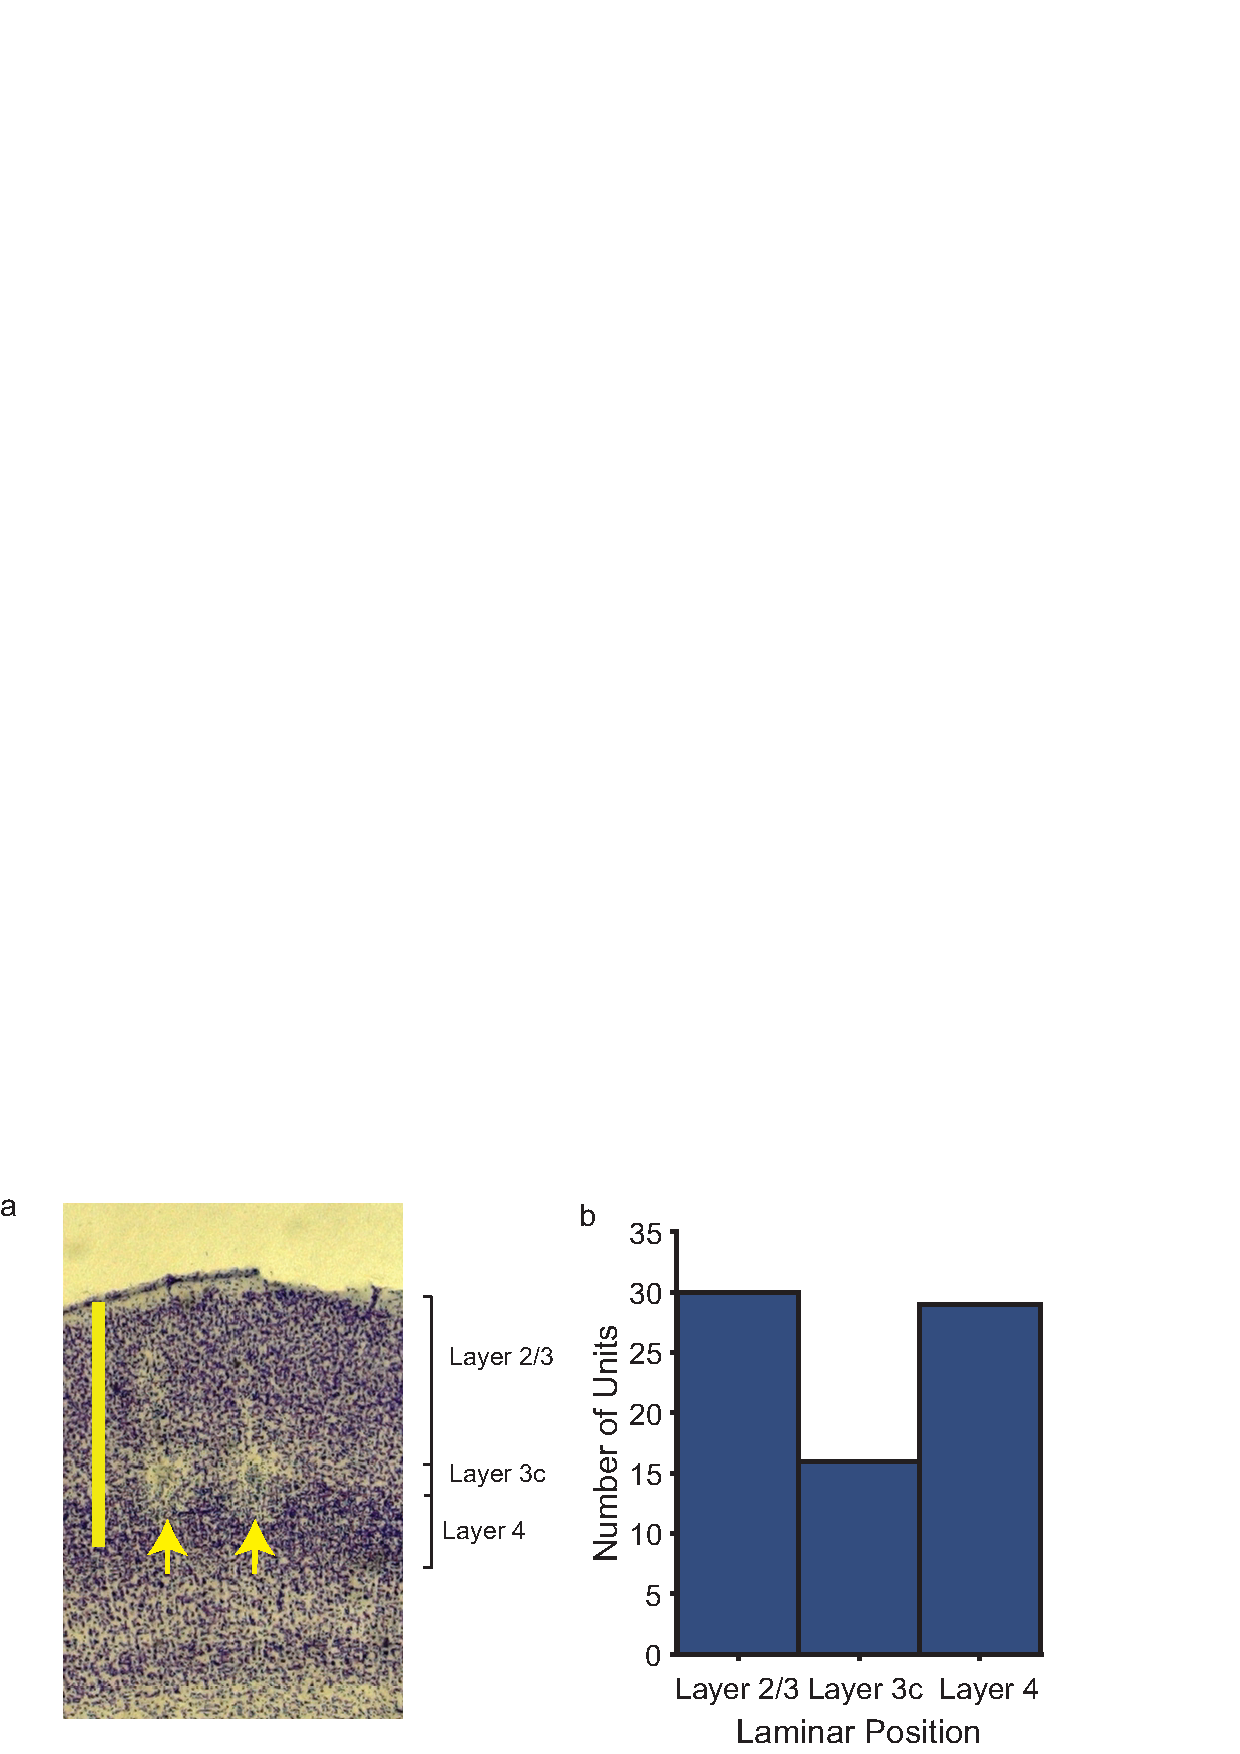
\includegraphics[width=\linewidth]{ShrewV1/LaminarPosition.jpg}
	\caption{The distribution of laminar positions from which we recorded. a) A photomicrograph of the tree shrew primary visual cortex with layers 2/3, 3c and 4 marked. The two arrows point to two lesions made in layer 3c of two separate tracks. The scale bar is 1 mm. b) Histogram showing the number of neurons recorded from each of the layers.}
	\label{fig:lp}
\end{figure} 

\subsubsection{Distribution of the circular variance}

The distribution of circular variances for neurons in the three layers, calculated from their responses to thin moving bars are shown in fig \ref{fig:cv}. The median CV of layer 2/3 neurons was 0.59 (n=28; 95\% CI= [0.32, 0.68]) ; that of layer 3c was  0.87 (n= 16; 95\% CI=[0.68, 0.91]) and that of layer 4 was 0.88 (n=29; 95\% CI=[0.84, 0.90 ]). The three distributions were significantly different from each other (p$<$0.001, Kruskal-Wallis test). Post-hoc tests revealed that there was a statistically significant distribution between the distribution of CVs of neurons in layer 2/3 and layer 3c (Mann-Whitney U test, z=2.37; p$<$0.01) and between layer 2/3 and layer 4 (Mann-Whitney U test, z= 3.58, p$<$0.001). The difference between the distributions of CV of layer 3c neurons and layer 4 neurons was not statistically significant (Mann-Whitney U test, z= 0.67; p=0.25). 
	\begin{figure}[H]
	
	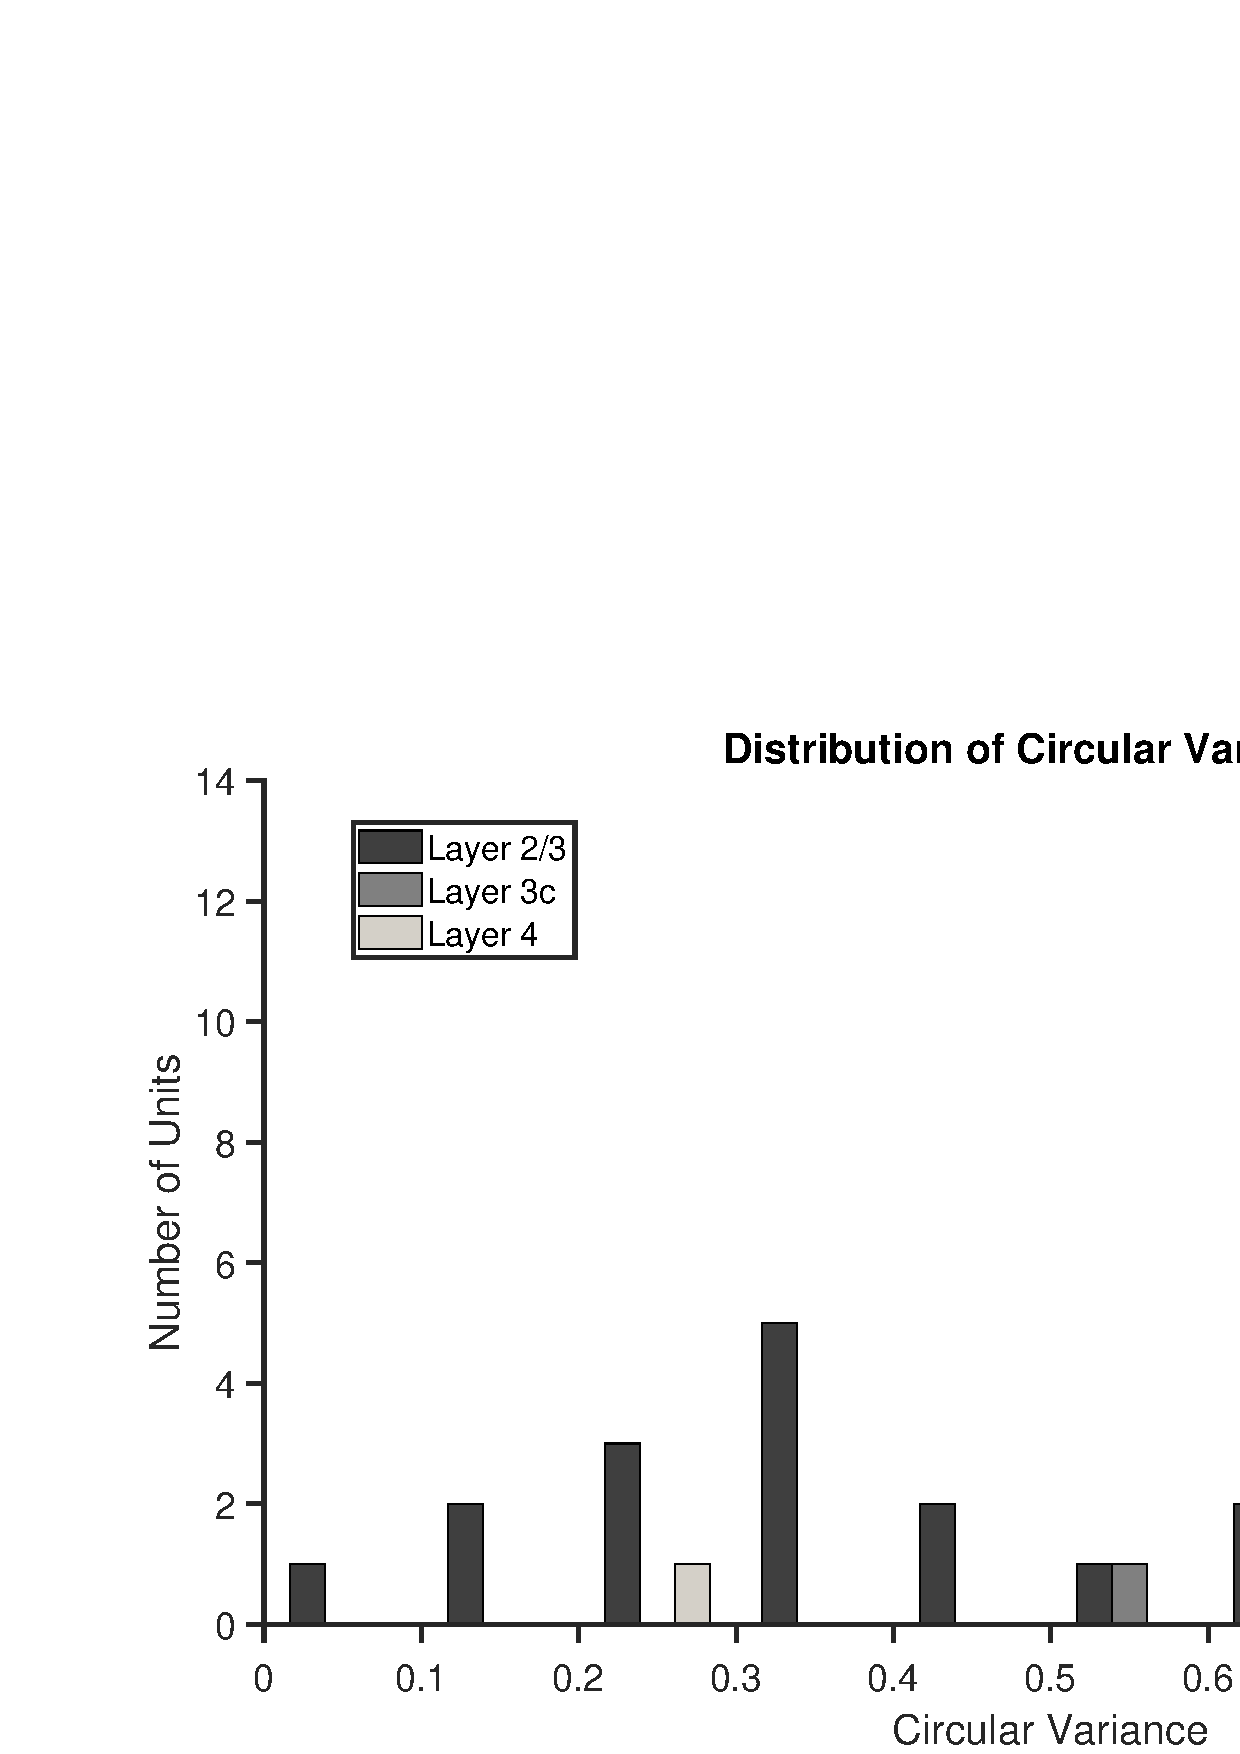
\includegraphics[width=\linewidth]{ShrewV1/cv_lamina_2_bw.jpg}
	\caption{The distribution of circular variance of neurons of the shrew V1.}
	\label{fig:cv}
\end{figure} 

\subsubsection{Circular mean of neurons}

According to our scheme of orientation selectivity in the tree shrews, layer 2/3 neurons inherit their orientation selectivity from layer 4 neurons which are biased for orientation. Here we test this hypothesis. Further, neurons in the tree shrew Layer 4 were thought to be untuned to orientation. However, recent studies, along with our own results in fig \ref{fig:cv} show that these neurons show orientation biases. Hence, we also wanted to determine if the orientation columns reported in the shrew Layer 2/3 extended to layer 4. As a result, we took the absolute difference between the circular means of each layer 2/3 neurons and subsequent neurons recorded from layers 3c and 4. These are shown in fig \ref{fig:cmdiff}.
	\begin{figure}[H]
	
	\includegraphics[width=\linewidth]{ShrewV1/cmdiff.jpg}
	\caption{The absolute difference between the circular mean of the first layer 2/3 neurons in each track and subsequent neurons from layer 3c and layer 4 in each track.}
	\label{fig:cmdiff}
	\end{figure}

Instead of the expected unimodal distribution where most neurons in a track were tuned to the same orientation, our results showed a bimodal distribution with approximately half the neurons tuned to the same orientation as the layer 2/3 neuron while the other half was tuned to an orientation that was 65$^o$ away.

We then split the distribution in two groups: pairs of neurons that were tuned to orientations less that 45$^o$ (group 1) apart and pairs tuned to orientation greater than 45$^o$ apart (Group 2). We then looked at whether the difference of was between the layer 2/3 neuron and layer 3c neurons or between layer 2/3 neuron and layer 4 neurons. These results are shown in fig \ref{fig:cmlayer}. We found that in group 1, the majority of the difference pairs were between layer 2/3 and layer 4 neurons (N=15; Binomial Distribution, p=0.04). In group 2, majority of the difference pairs were between layer 2/3 and layer 3c neurons (N=22; Binomial Distribution, p=0.04)

	\begin{figure}[H]
		
		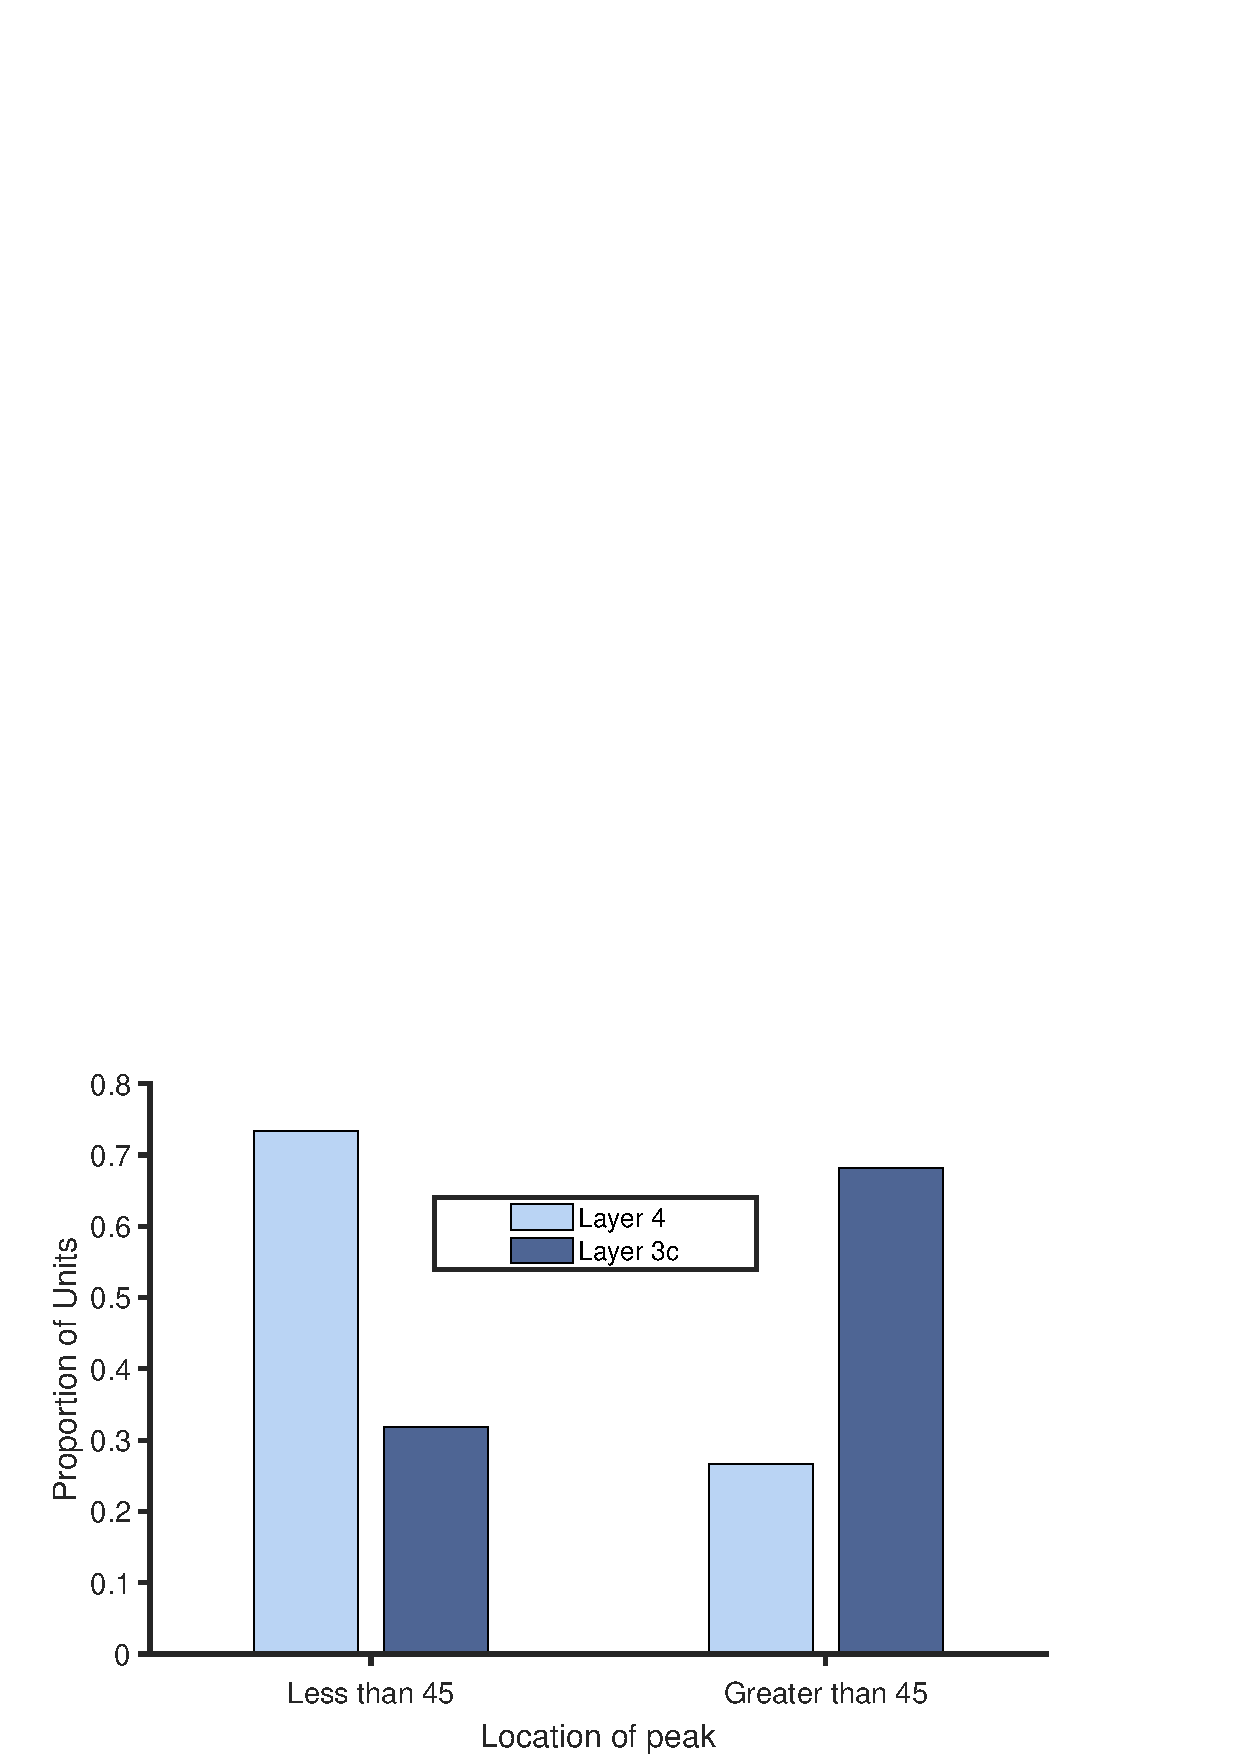
\includegraphics[width=\linewidth]{ShrewV1/cmlayer.jpg}
		\caption{The proportion of neurons from layers 3c and layer 4 with absolute differences greater and lesser than 45$^o$.}
		\label{fig:cmlayer}
	\end{figure}

In order to ensure that the second peak we observed in fig \ref{fig:cmdiff} wasn't due to track angles, we undertook a simulation experiment (see Methods, Random Simulation). We found that for the shortest distance between the layer 2/3 and layer 4 neurons in our sample (50 mm), there was a high probability of getting an absolute difference of 0 but this probability decreased steadily. For the greatest distance in our sample (300 mm), the probability of obtaining the same orientation diminished significantly. While there was a general trend towards getting neurons that were tuned 90$^o$ apart but there was no specific bias for a difference of 65$^o$. The highest probability of obtaining a peak at 65$^o$ was when distance was set at 250 mm (p=0.045).
		\begin{figure}[H]
		
		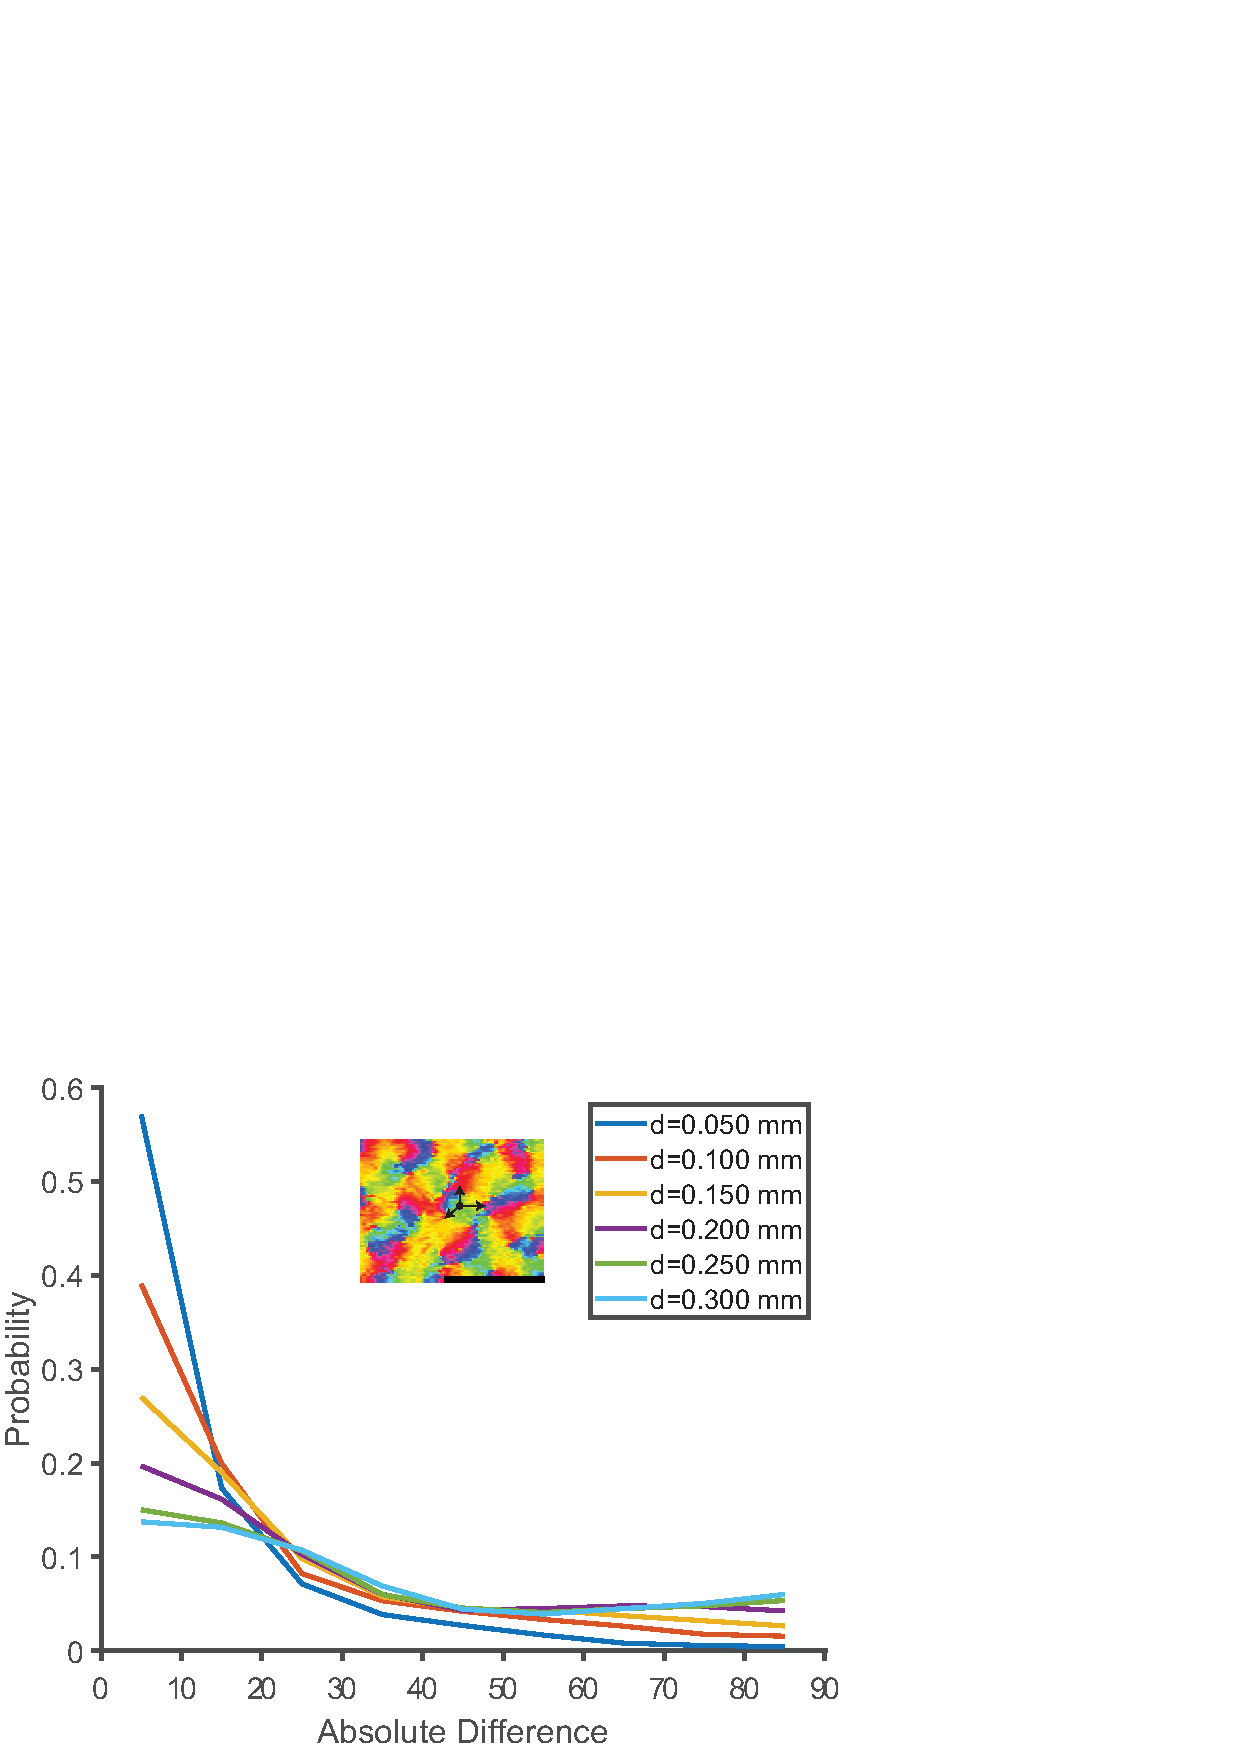
\includegraphics[width=\linewidth]{ShrewV1/simulation.jpg}
		\caption{Results of a simulation experiment: The orientation tuning map (inset) was taken from Bosking et al., 1997. On this map, points were randomly placed and the orientation of 1000 pixels randomly selected at one of the distances in the legend was subtracted from the original data point. For each distance, the distribution of absolute differences for the 1000 pixels are shown by the lines in the graph. Black line is 1mm.}
		\label{fig:sim}
	\end{figure}

\subsubsection{Spatial Frequency Tuning of neurons}

The distribution of the low cut-off, preferred and high cut-off spatial frequencies of the neurons in layer 2/3 and layer 4are shown in fig \ref{fig:sftuning}. Results from only these two layers are shown as we propose that the orientation selectivity of layer 2/3 neurons arise predominantly from layer 4 neurons. We found no significant differences between the spatial frequency tuning between the two layers, although layer 2/3 neurons show high spatial frequency attenuation. When the bandwidth of spatial frequency tuning in octaves was calculated, we found that the layer 2/3 neurons showed slightly sharper tuning (Median layer 2/3 b$_{oct}$= 2.2; n=16; Median layer 4 b$_{oct}$=2.3; n=9). This difference was however not statistically significant (Mann-Whitney U test; z=-1.18; p=0.24).

		\begin{figure}[H]
		
		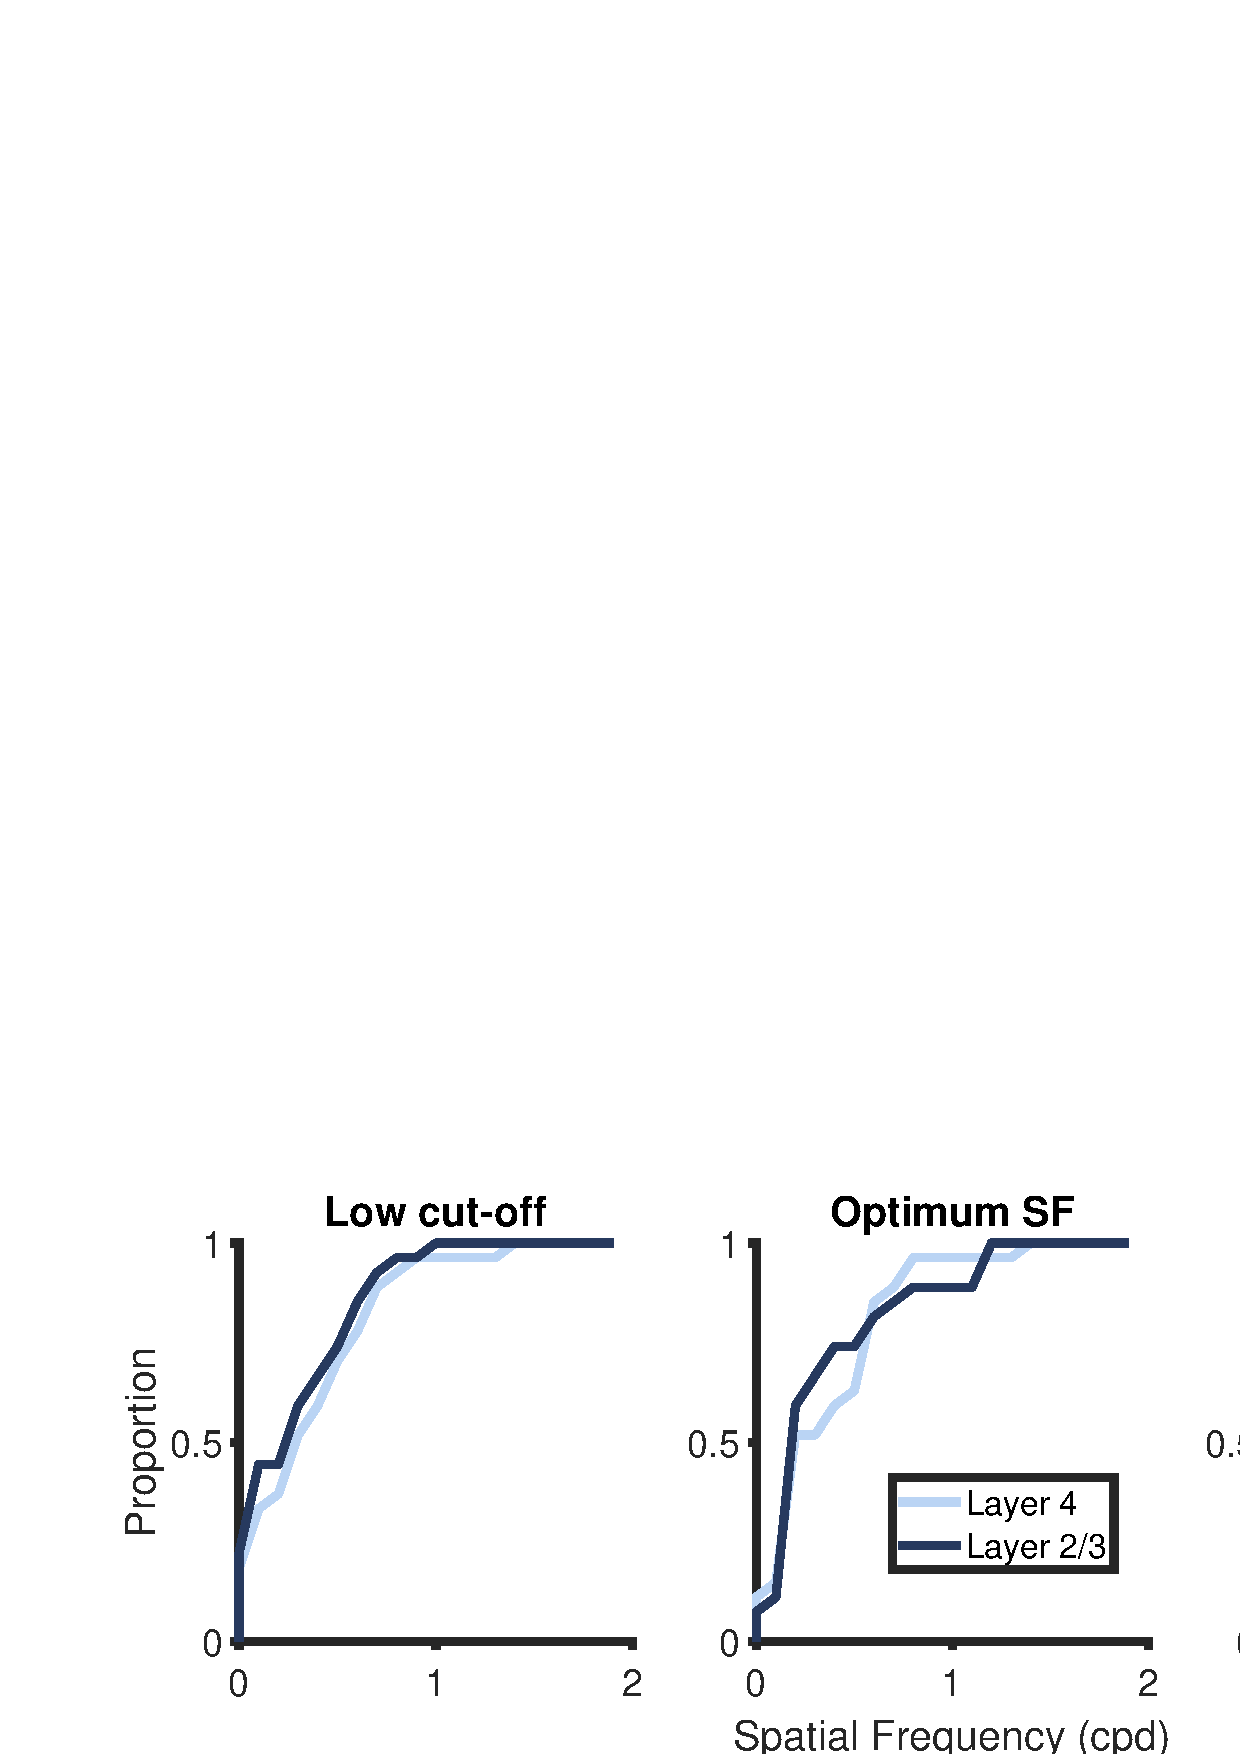
\includegraphics[width=\linewidth]{ShrewV1/sftuning_neurons_2.jpg}
		\caption{The cumulative distribution of the spatial frequency tuning of neurons in layers 2/3, 3c and 4 of the Shrew V1.}
		\label{fig:sftuning}
	\end{figure}

In 18 individual tracks, we compared the spatial frequency and orientation tuning of the layer 2/3 neuron to that of the first layer 4 neuron we encountered. The results of this analysis is shown in fig \ref{fig:sfsum}. The result from an example neuron is shown in parts a and b. Fig \ref{fig:sfsum}a shows that spatial frequency tuning curve of layer 2/3 neuron and that of the layer 4 neuron to optimum and orthogonal orientation. We expected that the optimum spatial frequency of the layer 2/3 neuron and the spatial frequency at which the layer 4 neurons was most tuned for orientation would be similar. We found that this relation held true only in 3 of our 18 tracks. In most of the tracks the maximum OSI of the layer 4 neuron occured at much higher spatial frequencies when compared to the optimum spatial frequency of the layer 2/3 neuron as demonstrated by the data points skewed closer to the y-axis.
	\begin{figure}[H]
	
		\includegraphics[width=\linewidth]{ShrewV1/sfsummary.jpg}
		\caption{The cumulative distribution of the spatial frequency tuning of neurons in layers 2/3, 3c and 4 of the Shrew V1.}
		\label{fig:sfsum}
	\end{figure}

\section{Discussion}
\section{Conclusion}